\documentclass[11pt]{article}

\usepackage[letterpaper,margin=0.75in]{geometry}
\usepackage{booktabs}
\usepackage{graphicx}
\usepackage{listings}

\setlength{\parindent}{1.4em}

\begin{document}

\lstset{
  language=Python,
  basicstyle=\small,          % print whole listing small
  keywordstyle=\bfseries,
  identifierstyle=,           % nothing happens
  commentstyle=,              % white comments
  stringstyle=\ttfamily,      % typewriter type for strings
  showstringspaces=false,     % no special string spaces
  numbers=left,
  numberstyle=\tiny,
  numbersep=5pt,
  frame=tb,
}

\title{Lab 1 Report}

\author{Jonathan George}

\date{January 27th, 2015}

\maketitle

This report covers the findings from simulating a network using a packet-level, event-driven simulator. Using the simulator, some basic networks were setup and used to verify delay and loss statitics. As well, basic queueing theory was examined, showing how queueing delay can grow exponentially as utilization approaches 100\%. 

The code for this project can be found at https://github.com/qzcx/bene

\section{Two Nodes - Part 1}

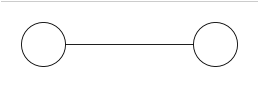
\includegraphics{TwoNodes.png}

In this first section, a simple two node network was simulated. The bandwidth of the links was set to 1 Mbps with a propagation delay of 1 second. A single packet of 1000 bytes was sent at time 0.

\begin{lstlisting}
class DelayHandler(object):

    def receive_packet(self,packet):
        print Sim.scheduler.current_time(),"\t",packet.ident,"\t",packet.created,"\t",\
            Sim.scheduler.current_time() - packet.created,packet.transmission_delay,"\t",\
            packet.propagation_delay,"\t",packet.queueing_delay

_1MBPS = 1000000
_1GBPS = _1MBPS * 1000

def run():
    print "time\t","ident\t","created\t", "sent_at\t", "Dtrans\t", "Dprop\t", "Dqueue\t"
    Sim.scheduler.run()

def twoNodeSetUp():
    # parameters
    Sim.scheduler.reset()

    # setup network
    net = Network('twoNodes.txt')

    # setup routes
    n1 = net.get_node('n1')
    n2 = net.get_node('n2')
    n1.add_forwarding_entry(address=n2.get_address('n1'),link=n1.links[0])
    n2.add_forwarding_entry(address=n1.get_address('n2'),link=n2.links[0])

    # setup app
    d = DelayHandler()
    net.nodes['n2'].add_protocol(protocol="delay",handler=d)
    return n1,n2

"""
Set the bandwidth of the links to 1 Mbps, with a propagation delay of 1 second. 
Send one packet with 1000 bytes from n1 to n2 at time 0.
"""
def twoNodes_1():
    n1,n2 = twoNodeSetUp()

    n1.links[0].bandwidth = _1MBPS
    n2.links[0].bandwidth = _1MBPS
    n1.links[0].propagation = 1;
    n2.links[0].propagation = 1;

    # send one packet
    p = packet.Packet(destination_address=n2.get_address('n1'),
                        ident=1,protocol='delay',length=1000)
    Sim.scheduler.add(delay=0, event=p, handler=n1.send_packet)
    # run the simulation
    run()
\end{lstlisting}

The output from this program was:

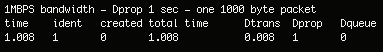
\includegraphics{twoNode-1.png}

From this output we can see that the propegation time was 1 second and the transmission time was 8 milliseconds. This matches what we should expect since a bandwidth of 1 Mbps would take 1 microsecond per bit. Therefore to process the 1000 byte (or 8000 bit) package, we should expect it to take 8 milliseconds.


\section{Two Nodes - Part 2}

For this section we descreased the bandwidth to 100 bps and a propegation delay of 10 ms. 

\begin{lstlisting}
"""
Set the bandwidth of the links to 100 bps, with a propagation delay of 10 ms. 
Send one packet witih 1000 bytes from n1 to n2 at time 0.
"""
def twoNodes_2():
    n1,n2 = twoNodeSetUp()

    n1.links[0].bandwidth = 100
    n2.links[0].bandwidth = 100
    n1.links[0].propagation = 0.010 #10 ms
    n2.links[0].propagation = 0.010 #10 ms

    # send one packet
    p = packet.Packet(destination_address=n2.get_address('n1'),
                        ident=1,protocol='delay',length=1000)
    Sim.scheduler.add(delay=0, event=p, handler=n1.send_packet)

    run()


\end{lstlisting}
The output from this program was

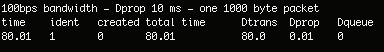
\includegraphics{twoNode-2.png}

We can see here that the transmission delay inceased to 80 seconds. By decreasing the bandwidth by a factor of 10000, our transmission delay increased by the same factor. 

\section{Two Nodes - Part 3}

In this section, we will show the effects of queuing delay on a two node system. We will set the bandwidth of the links to 1 Mbps, with a propagation delay of 10 ms. Then we will send 3 packets together at time 0 seconds. Then after those packets are passed through the system, we will send a fourth packet to show the typical isolated case.

\begin{lstlisting}
"""
Set the bandwidth of the links to 1 Mbps, with a propagation delay of 10 ms. 
Send three packets from n1 to n2 at time 0 seconds, then one packet at time 2 seconds. 
All packets should have 1000 bytes.
"""
def twoNodes_3():
    n1,n2 = twoNodeSetUp()

    n1.links[0].bandwidth = _1MBPS
    n2.links[0].bandwidth = _1MBPS
    n1.links[0].propagation = 0.010 #10 ms
    n2.links[0].propagation = 0.010 #10 ms

    # send three packet
    p = packet.Packet(destination_address=n2.get_address('n1'),
                        ident=1,protocol='delay',length=1000)
    Sim.scheduler.add(delay=0, event=p, handler=n1.send_packet)
    p = packet.Packet(destination_address=n2.get_address('n1'),
                        ident=1,protocol='delay',length=1000)
    Sim.scheduler.add(delay=0, event=p, handler=n1.send_packet)
    p = packet.Packet(destination_address=n2.get_address('n1'),
                        ident=1,protocol='delay',length=1000)
    Sim.scheduler.add(delay=0, event=p, handler=n1.send_packet)

    #One more at t=2
    p = packet.Packet(destination_address=n2.get_address('n1'),
                        ident=1,protocol='delay',length=1000)
    Sim.scheduler.add(delay=2, event=p, handler=n1.send_packet)

    run()
\end{lstlisting}
The output of the progam:

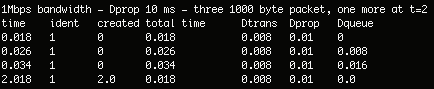
\includegraphics[width=11cm]{twoNode-3.png}

We can see that like the first setup, the transmission delay was 8 milliseconds. However, in this case the second and third packet had to wait for the packets which were in front of them. This caused a queuing delay of 8 milliseconds and 16 milliseconds respectively. This also shows the pipeline nature of network links. The queuing delay was only dependent on the propegation delay and not the transmission delay. 

Also as expected the packet sent 2 seconds after the first 3 had 0 queuing theory delay and a total time equal to the first packet.

\section{Three Nodes - Two Fast Links}



In this next section we will show the relationship between multiple links. We will set up three nodes and vary the bandwidths of the second link in the node.

In the first simulation we will use two nodes which have the same bandwidth of 1 Mbps and send 1000 packets of size 1000 Bytes. We will also compare this to the situation where we have 1 Gbps links.

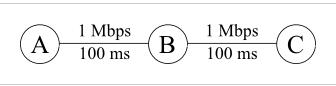
\includegraphics{ThreeFast.png}

\begin{lstlisting}
def threeNodeSetup():
    # parameters
    Sim.scheduler.reset()

    # setup network
    net = Network('threeNodes.txt')

    # setup routes
    n1 = net.get_node('n1')
    n2 = net.get_node('n2')
    n3 = net.get_node('n3')
    n1.add_forwarding_entry(address=n2.get_address('n1'),link=n1.links[0])
    n1.add_forwarding_entry(address=n3.get_address('n2'),link=n1.links[0])
    n2.add_forwarding_entry(address=n1.get_address('n2'),link=n2.links[0])
    n2.add_forwarding_entry(address=n3.get_address('n2'),link=n2.links[1])
    n3.add_forwarding_entry(address=n1.get_address('n2'),link=n3.links[0])
    n3.add_forwarding_entry(address=n2.get_address('n3'),link=n3.links[0])

    # setup app
    d = DelayHandler3Node()
    net.nodes['n3'].add_protocol(protocol="delay",handler=d)
    
    return n1,n2,n3

#def sendPacket(src, dest):


"""
Two fast links - 1MBPS - 100ms

Node A transmits a stream of 1 kB packets to node C. 
How long does it take to transfer a 1 MB file, divided into 1 kB packets, from A to C? 
Which type of delay dominates?
"""
def fastLinks():
    n1,n2,n3 = threeNodeSetup()

    n1.links[0].bandwidth = _1MBPS
    n2.links[0].bandwidth = _1MBPS
    n2.links[1].bandwidth = _1MBPS
    n3.links[0].bandwidth = _1MBPS

    n1.links[0].propagation = 0.100 #100 ms
    n2.links[0].propagation = 0.100 #100 ms
    n2.links[1].propagation = 0.100 #100 ms
    n3.links[0].propagation = 0.100 #100 ms



    for i in range(0,1000):
        p = packet.Packet(destination_address=n3.links[0].address,
                        ident=i,protocol='delay',length=1000)
        Sim.scheduler.add(delay=0, event=p, handler=n1.send_packet)

    Sim.scheduler.run()

"""
If both links are upgraded to a rate of 1 Gbps, 
how long does it take to transfer a 1 MB file from A to C?
"""
def fasterLinks():
    n1,n2,n3 = threeNodeSetup()

    n1.links[0].bandwidth = _1GBPS
    n2.links[0].bandwidth = _1GBPS
    n2.links[1].bandwidth = _1GBPS
    n3.links[0].bandwidth = _1GBPS

    n1.links[0].propagation = 0.100 #100 ms
    n2.links[0].propagation = 0.100 #100 ms
    n2.links[1].propagation = 0.100 #100 ms
    n3.links[0].propagation = 0.100 #100 ms

    for i in range(0,1000):
        p = packet.Packet(destination_address=n3.links[0].address,
                        ident=i,protocol='delay',length=1000)
        Sim.scheduler.add(delay=0, event=p, handler=n1.send_packet)

    Sim.scheduler.run()
\end{lstlisting}
For the 1 Mbps links we get the output: 

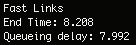
\includegraphics{3fast.png}

We can see from these results that this matches our anaylsis of the two node setup with the exception that there is an extra 0.1 milliseconds due to the extra length the packet must travel. By sending 1000 packets, it increased the transmission delay by a factor of 1000. However, similar to the third two node situation only the transmission delay causes queuing delay. We can see from this example, that the transmission delay dominates the propagation delay.

For the 1 Gbps links we get the output:

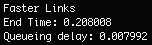
\includegraphics{3faster.png}

We can see that both the transmission delay and the queuing delay decreased by a factor of 1000. This is as expected.


\section{Three Nodes - One Slow link}



In this last situation, we will decrease the second link's bandwidth to 256 kbps. This will cause queuing delay in the the second node because it's arrival rate will be greater than it's departure rate.

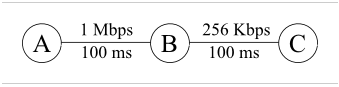
\includegraphics{ThreeSlow.png}

\begin{lstlisting}
"""
One fast link and one slow link - 1MBPS/256KBPS - 100ms

Node A transmits 1000 packets, each of size 1 kB, to node C. 
How long would it does it take to transfer a 1 MB file, divided into 1 kB packets, from A to C?
"""
def slowLink():
    n1,n2,n3 = threeNodeSetup()

    n1.links[0].bandwidth = _1MBPS
    n2.links[0].bandwidth = _1MBPS
    n2.links[1].bandwidth = 256*1000 #256Kbps
    n3.links[0].bandwidth = 256*1000 #256Kbps

    n1.links[0].propagation = 0.100 #100 ms
    n2.links[0].propagation = 0.100 #100 ms
    n2.links[1].propagation = 0.100 #100 ms
    n3.links[0].propagation = 0.100 #100 ms

    for i in range(0,1000):
        p = packet.Packet(destination_address=n3.links[0].address,
                        ident=i,protocol='delay',length=1000)
        Sim.scheduler.add(delay=0, event=p, handler=n1.send_packet)
    Sim.scheduler.run()
\end{lstlisting}

Our results were:

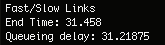
\includegraphics{3slow.png}

We can see that our expectations were met and the delay increased by a factor of 4. 
The total propagation delay should be 200 ms. The first link contributes 8 ms of transmision delay and then the second link takes 8000/256Kbps per packet. This totals to 31.458 seconds which matches our simulator output

\section{Queueing Theory}

In this final section we will simulate basic queuing theory, showing that as utility approaches 100\%, the queueing delay approaches infinite. 

The code below is based off of delay.py written by Dr. Zapalla
\begin{lstlisting}
import sys
sys.path.append('..')

from src.sim import Sim
from src import node
from src import link
from src import packet

from networks.network import Network

import random as random1

import optparse

import matplotlib
matplotlib.use('Agg')
from pylab import *

class Generator(object):
    def __init__(self,node,destination,load,duration):
        self.node = node
        self.load = load
        self.duration = duration
        self.start = 0
        self.ident = 1
        self.destination = destination

    def handle(self,event):
        # quit if done
        now = Sim.scheduler.current_time()
        if (now - self.start) > self.duration:
            return

        # generate a packet
        self.ident += 1
        p = packet.Packet(destination_address=self.destination,ident=self.ident,protocol='delay',length=1000)
        Sim.scheduler.add(delay=0, event=p, handler=self.node.send_packet)
        # schedule the next time we should generate a packet
        Sim.scheduler.add(delay=random1.expovariate(self.load), event='generate', handler=self.handle)




class DelayHandler(object):
    def receive_packet(self,packet):
        global count
        global tot_delay
        tot_delay += packet.queueing_delay
        count += 1

def calc_avg_delay(loadFactor):
    # parameters
    Sim.scheduler.reset()

    # setup network
    net = Network('../networks/one-hop.txt')

    # setup routes
    n1 = net.get_node('n1')
    n2 = net.get_node('n2')
    n1.add_forwarding_entry(address=n2.get_address('n1'),link=n1.links[0])
    n2.add_forwarding_entry(address=n1.get_address('n2'),link=n2.links[0])

    # setup app
    d = DelayHandler()
    net.nodes['n2'].add_protocol(protocol="delay",handler=d)

    # setup packet generator
    destination = n2.get_address('n1')
    max_rate = 1000000/(1000*8)
    load = loadFactor*max_rate
    g = Generator(node=n1,destination=destination,load=load,duration=10)
    Sim.scheduler.add(delay=0, event='generate', handler=g.handle)
    
    # run the simulation
    Sim.scheduler.run()
    print "average =", tot_delay/count,"count =",count

    return tot_delay/count

def plot_results(trials,results):
    """ Create a line graph of an equation. """
    clf()

    plot(trials,results)

    
    x = np.arange(0,1,0.01)
    u = 1000000.0/(1000.0*8.0)
    plot(x,(1/(2*u))*x/(1-x),label='Theory',color="green")

    xlabel('utilization')
    ylabel('1/(2u) x p/(1-p)')
    savefig('equation.png')


if __name__ == '__main__':
    trials = [.10,.20,.30,.40,.50,.60,.70,.80,.90,.95,.97,.98,]
    results = []
    global count
    global tot_delay
    tot_delay = 0
    count = 0
    for load in trials:
        results.append(calc_avg_delay(load))
        count = 0
        tot_delay = 0
    plot_results(trials,results)
\end{lstlisting}
The code above uses a two node simulator and a random generator to supply a certain load to the simulator. By simulating, different loads we can see how system's queuing delay changes based on utilization. 

The theoretical curve of 1/(2*mu)*rho/(1-rho) is used as a comparison. 

Our final result shown below, shows that our simulator matches the expected equation. Although we did notice that the results of the generator did vary. It would probably be better in the future to do many trials and average those results to see a more smooth curve. Overall for this experiement these results are satisifactory because we can still see the general trend clearly. 

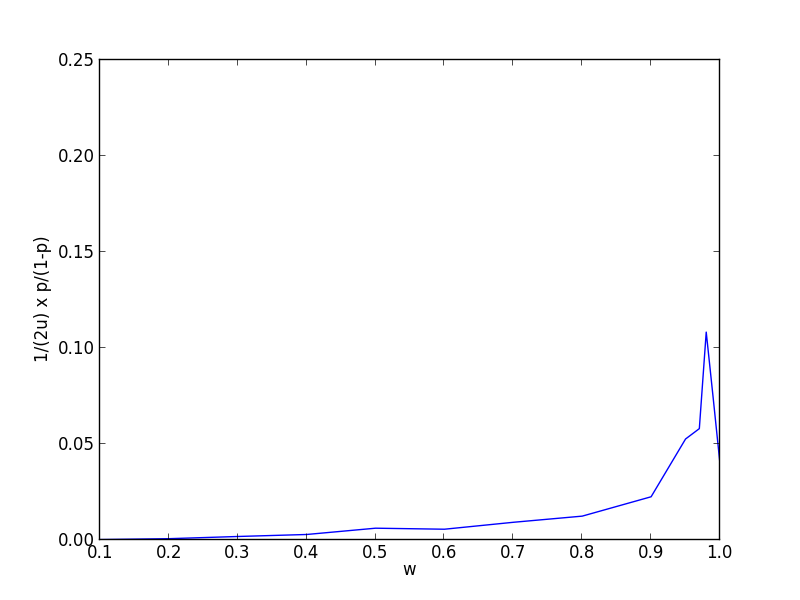
\includegraphics{equation.png}

\end{document}